\section{Algorithm: SLMS}
\label{sec:algorithm}

SLMS is a certificate-based stabilizer-aware tree-decomposition criterion with local quasiprobability sampling. In the main theorem (Section~\ref{sec:main-theorem}) it is stated only for locally marginalizable resource-decomposition networks, so every message has a certified active boundary and a certified burden \(\Gamma_b\). The proved algorithm estimates a scalar root probability; message tables are an implementation strategy, not part of the theorem statement.

\begin{figure}[t]
\centering
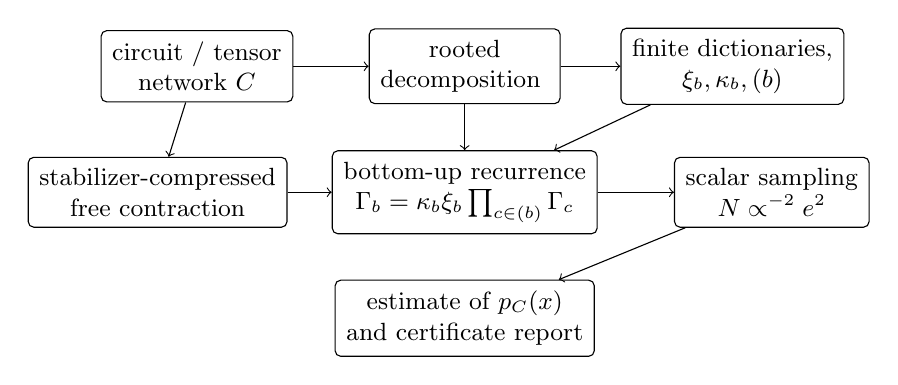
\begin{tikzpicture}[node distance=1.4cm, every node/.style={draw, rounded corners=2pt, align=center, inner sep=4pt, font=\small}]
\node (input) {circuit / tensor\\network \(C\)};
\node[right of=input, xshift=2.0cm] (decomp) {rooted\\decomposition \(\T\)};
\node[right of=decomp, xshift=2.0cm] (cert) {finite dictionaries,\\\(\xi_b,\kappa_b,\Act(b)\)};
\node[below of=decomp, yshift=-0.2cm] (rec) {bottom-up recurrence\\\(\Gamma_b=\kappa_b\xi_b\prod_{c\in\Act(b)}\Gamma_c\)};
\node[right of=rec, xshift=2.5cm] (sample) {scalar sampling\\\(N\propto \eps^{-2}e^{2\Lammsg}\)};
\node[left of=rec, xshift=-2.5cm] (stab) {stabilizer-compressed\\free contraction};
\node[below of=rec, yshift=-0.2cm] (out) {estimate of \(p_C(x)\)\\and certificate report};
\draw[->] (input) -- (decomp);
\draw[->] (decomp) -- (cert);
\draw[->] (cert) -- (rec);
\draw[->] (decomp) -- (rec);
\draw[->] (input) -- (stab);
\draw[->] (stab) -- (rec);
\draw[->] (rec) -- (sample);
\draw[->] (sample) -- (out);
\end{tikzpicture}
\caption{SLMS certificate and scalar-estimation pipeline. The active-child recurrence is a junction-tree-style collect recurrence equipped with stabilizer compression and certified local quasiprobability costs.}
\label{fig:slms-pipeline}
\end{figure}

\subsection{Inputs and message objects}

Figure~\ref{fig:slms-pipeline} summarises the pipeline from input network and decomposition through the active-child recurrence to the scalar sampler. The inputs are:
\begin{itemize}[leftmargin=1.2cm]
\item a circuit or tensor network \(C\) and output event \(x\);
\item a rooted tree decomposition \(\T=(T,\beta)\);
\item an effective-boundary certificate giving \(\weff\);
\item a resource assignment \(\alpha:\R(C)\to V(T)\);
\item local free-tensor decompositions and bag costs \(\xi_b\);
\item certified local coefficient-map norm factors \(\kappa_b\ge 1\);
\item active-child sets \(\Act(b)\subseteq\ch(b)\);
\item an additive error \(\eps>0\) and failure probability \(\delta\in(0,1)\).
\end{itemize}

A message object emitted by a bag \(b\) contains:
\begin{itemize}[leftmargin=1.2cm]
\item the active boundary index set and dense dimension \(D_b\le 2^{\weff}\);
\item a stabilizer/free symbolic representation for the compressed boundary degrees of freedom;
\item a dense table for active boundary entries when needed;
\item the certified burden \(\Gamma_b\);
\item the local sampling distribution over the bag expansion and active child representatives.
\end{itemize}

\subsection{Scalar versus table estimation}

The main theorem analyzes scalar root estimation. In this mode SLMS samples a complete active quasiprobability assignment along the certified recurrence and contracts the corresponding free/stabilizer network to one scalar estimator for \(p_C(x)\). The second moment is bounded by the square of the relevant \(\ell_1\) message cost, hence by \(\exp(2\Lammsg)\).

An implementation may instead estimate intermediate active-boundary message tables entrywise. Then each table has dimension \(D_b\le 2^{O(\weff)}\), each entry needs its own accuracy budget, and a union bound or deterministic error-propagation argument is required over all table entries and all bags. These costs are the source of the \(2^{O(\weff)}\) factor in the theorem. The paper uses scalar estimation for the proof statement and table estimation as an implementation option.

\subsection{Pseudocode}

\begin{center}
\fbox{\begin{minipage}{0.93\linewidth}
\textbf{SLMS: Separator-Local Magic Simulator}

\vspace{0.4em}
\textbf{Input:} \(C,x,\T,\alpha,\{\xi_b\},\{\kappa_b\},\{\Act(b)\},\weff,\eps,\delta\).

\textbf{Output:} Estimate \(\widehat p\) of \(p_C(x)\).

\begin{enumerate}[leftmargin=1.0cm]
\item Verify the contraction graph and the rooted tree decomposition for the scalar \(p_C(x)\).
\item Compress free stabilizer regions and record active boundary dimensions \(D_b\le 2^{\weff}\).
\item For each bag \(b\), form a certified local quasiprobability expansion of cost \(\xi_b\).
\item Compute message burdens bottom-up:
\[
\Gamma_b\leftarrow \kappa_b\xi_b\prod_{c\in\Act(b)}\Gamma_c .
\]
\item Repeat \(N=O(\eps^{-2}\exp(2\Lammsg)\log(1/\delta))\) scalar samples:
\begin{enumerate}[label*=\arabic*.]
\item sample only the local bag expansions and active child representatives appearing in the certified recurrence;
\item treat inactive child messages as deterministic inputs already marginalized at their parent bags;
\item contract the sampled free network using stabilizer compression and dense active boundary dimension at most \(2^{O(\weff)}\);
\item return one signed scalar estimator for \(p_C(x)\).
\end{enumerate}
\item Aggregate the scalar samples, for example by median-of-means, and return \(\widehat p\) with its confidence interval.
\end{enumerate}
\end{minipage}}
\end{center}

\subsection{Certification procedures}
\label{sec:certification}

The theorem is certificate-based, but the certificates are explicit finite checks. For finite tensor networks of bounded local dimension, the following procedures give checkable sufficient conditions. They may be conservative: failing a check means that the child or boundary is marked active, not that the circuit is hard.

\paragraph{Free-region detection.}
Build the induced subgraph on tensors labelled free: stabilizer states, Clifford maps, Pauli effects, computational-basis stochastic maps, and previously certified free mixtures. Connected components of this subgraph are candidate free regions. Boundary legs incident to resource tensors or active child messages are recorded as active legs; all other stabilizer boundary data are stored symbolically.

\paragraph{Effective-width upper bound.}
For each separator \(e\), compute the dense boundary dimension before compression, \(D_e^{\mathrm{TN}}\). Then remove boundary degrees of freedom that the free-region certificate represents purely by stabilizer tableaux, affine symplectic constraints, or normalized classical stochastic stabilizer messages. The remaining dense dimension \(D_e^{\mathrm{act}}\) gives
\[
\weff\le \max_e \log_2 D_e^{\mathrm{act}}.
\]
If the symbolic compression check fails, set \(D_e^{\mathrm{act}}=D_e^{\mathrm{TN}}\).

\paragraph{Inactive-child marginalization check.}
For a child \(c\) of \(b\), form the local map that contracts the message from \(c\) with the tensors at \(b\) that consume the child boundary, while leaving only the outgoing active boundary of \(b\) open. The child can be declared inactive if this map sends every normalized free representative in the certified child message class to a normalized free message or to a deterministic dense active-boundary table with certified \(\ell_1\) cost at most one. For constant-size boundaries this can be checked by enumerating stabilizer extreme points; for larger classical stochastic boundaries it reduces to checking nonnegative column sums.

\paragraph{Local \(\ell_1\)-nonexpansiveness.}
Represent the local contraction map, restricted to the finite list of free representatives appearing in the local and active-child decompositions, as a matrix \(L_b\) from coefficient vectors to outgoing message coefficients. A sufficient certificate is
\[
\norm{L_b}_{1\to 1}=\max_j\sum_i |(L_b)_{ij}|\le 1.
\]
If \(\norm{L_b}_{1\to 1}=L_b^\ast>1\), set \(\kappa_b=L_b^\ast\). If the norm is not certified, the conservative response is to mark the relevant child messages active or merge the local region into a larger certified bag.

\paragraph{Automatic active-child selection.}
Process bags bottom-up. For each child \(c\), attempt the inactive-child marginalization check. If it succeeds, set \(c\notin\Act(b)\). If it fails, set \(c\in\Act(b)\). This greedy rule gives a valid certificate when all local checks pass. It may not minimize \(\Lammsg\), since a globally better certificate may require a different decomposition or local normalization.

\begin{center}
\fbox{\begin{minipage}{0.93\linewidth}
\textbf{CERTIFY-LM: Conservative Local Marginalizability Certification}
\begin{enumerate}[leftmargin=1.0cm]
\item Label tensors as free or resource and identify connected free regions.
\item For each separator, compute \(D_e^{\mathrm{TN}}\) and a certified active dimension \(D_e^{\mathrm{act}}\).
\item For each bag \(b\), compute or import a local free-tensor quasiprobability expansion and cost \(\xi_b\).
\item For each child \(c\in\ch(b)\), run the inactive-child marginalization check.
\item Set \(\Act(b)\) to the children whose check fails.
\item For each bag, compute a certified \(1\to1\) norm factor \(\kappa_b\).
\item Return \(\weff\), \(\{\xi_b\}\), \(\{\kappa_b\}\), \(\{\Act(b)\}\), and \(\Lammsg\).
\end{enumerate}
\end{minipage}}
\end{center}

\subsection{Error allocation}

For a proof-level implementation, assign each message an entrywise accuracy
\[
\eta_b=\Theta\!\left(\frac{\eps}{\poly(|T|)2^{O(\weff)}}\right)
\]
and failure probability \(\delta_b=\delta/\poly(|T|)\). The certified local coefficient-norm factors in Definition~\ref{def:lm-network} are already included in \(\Gamma_b\), so message errors accumulate by at most the polynomial factor in the number of bags and active boundary dimension. This optional message-table mode gives the same dependence on \(\eps\), \(\delta\), \(\weff\), and the explicit sampling factor \(\exp(2\Lammsg)\) as the scalar theorem in Section~\ref{sec:main-theorem}, with additional implementation constants from table storage and error propagation.

\subsection{Baselines}

\begin{center}
\begin{tabular}{lll}
\toprule
Method & Dominant exponential & When it is relevant \\
\midrule
Dense tensor-network contraction & \(2^{O(\wTN)}\) & arbitrary tensors \\
Global quasiprobability sampling & \(\exp(2\Lambda_{\mathrm{glob}})\) & low total magic \\
Naive hybrid & \(2^{O(\weff)}\exp(2\Lambda_{\mathrm{glob}})\) & no local marginalization \\
SLMS (this paper) & \(2^{O(\weff)}\exp(2\Lammsg)\) & locally marginalizable networks \\
\bottomrule
\end{tabular}
\end{center}

The SLMS row is not automatically better than dense contraction. It is useful only when stabilizer compression gives \(\weff\ll\wTN\), or when the active-child recurrence gives \(\Lammsg\ll\Lambda_{\mathrm{glob}}\), or both. The scalar Monte Carlo variance bound gives the explicit sampling dependence \(\exp(2\Lammsg)\).
